%
% This is the LaTeX template file for lecture notes for CS294-8,
% Computational Biology for Computer Scientists.  When preparing 
% LaTeX notes for this class, please use this template.
%
% To familiarize yourself with this template, the body contains
% some examples of its use.  Look them over.  Then you can
% run LaTeX on this file.  After you have LaTeXed this file then
% you can look over the result either by printing it out with
% dvips or using xdvi.
%
% This template is based on the template for Prof. Sinclair's CS 270.

\documentclass[twoside]{ctexart}

\usepackage{listings,xcolor}
\usepackage{enumitem}
\usepackage{mathrsfs}
\usepackage{indentfirst} 
\usepackage{lstcustom}
\usepackage{ctex}
\usepackage{comment}
\usepackage{booktabs}
\usepackage{graphicx}
\usepackage{diagbox}
\usepackage{amsmath,amsfonts,graphicx,amssymb,bm,amsthm}
\usepackage{algorithm,algorithmicx}
\usepackage[noend]{algpseudocode}
\usepackage{fancyhdr}
\usepackage{tikz}
\usepackage{graphicx}
\usetikzlibrary{arrows,automata}
\usepackage{hyperref}

\setlength{\oddsidemargin}{0.25 in}
\setlength{\evensidemargin}{0.25 in}
\setlength{\topmargin}{-0.6 in}
\setlength{\textwidth}{6.5 in}
\setlength{\textheight}{8.5 in}
\setlength{\headsep}{0.75 in}
\setlength{\parindent}{0 in}
\setlength{\parskip}{0.1 in}

%
% The following commands set up the lecnum (lecture number)
% counter and make various numbering schemes work relative
% to the lecture number.
%
\newcounter{lecnum}
\newcounter{counter_exm}\setcounter{counter_exm}{1}
\newtheorem{theorem}{\hskip 1.7em 定理}
\newtheorem{lemma}[theorem]{\hskip 1.7em 引理}
\newtheorem{proposition}[theorem]{Proposition}
\newtheorem{claim}[theorem]{\hskip 1.7em 命题}
\newtheorem{corollary}[theorem]{\hskip 1.7em 推论}
\newtheorem{definition}[theorem]{\hskip 1.7em 定义}

\renewcommand{\emph}[1]{\begin{kaishu}#1\end{kaishu}}

\newenvironment{solution}{{\noindent\hskip 2em \bf 解 \quad}}


\renewenvironment{proof}{{\noindent\hskip 2em \bf 证明 \quad}}{\hfill$\qed$\par}
\newenvironment{example}{{\noindent\hskip 2em \bf 例 \arabic{counter_exm}\quad}}{\addtocounter{counter_exm}{1}\par}

\newenvironment{concept}[1]{{\bf #1\quad} \begin{kaishu}} {\end{kaishu}\par}

\newcommand\E{\mathbb{E}}

%
% The following macro is used to generate the header.
%

\newcommand{\lecture}[4]{
   \pagestyle{myheadings}
   \thispagestyle{plain}
   \newpage
   \setcounter{lecnum}{#1}
   \setcounter{page}{1}
   \noindent
   \begin{center}
   \framebox{
      \vbox{\vspace{2mm}
    \hbox to 6.28in { {\bf 计算机系统导论小班
                        \hfill 2020年秋季} }
       \vspace{4mm}
       \hbox to 6.28in { {\Large \hfill 课程回顾#1:#2  \hfill} }
       \vspace{2mm} 
       \hbox to 6.28in { {\it  \hfill 作者:#3} }
      \vspace{2mm}}
   }
   \end{center}
   \markboth{课程回顾#1:#2}{课程回顾#1:#2}
   {\bf 免责声明}:{\it 该笔记尚未进行正式出版物的通常审查,未经教师允许不能向课程外分发.}
   \vspace*{4mm}
}


\renewcommand{\cite}[1]{[#1]}
\def\beginrefs{\begin{list}%
        {[\arabic{equation}]}{\usecounter{equation}
         \setlength{\leftmargin}{2.0truecm}\setlength{\labelsep}{0.4truecm}%
         \setlength{\labelwidth}{1.6truecm}}}
\def\endrefs{\end{list}}
\def\bibentry#1{\item[\hbox{[#1]}]}

%Use this command for a figure; it puts a figure in wherever you want it.
%usage: \fig{NUMBER}{SPACE-IN-INCHES}{CAPTION}
\newcommand{\fig}[3]{
			\vspace{#2}
			\begin{center}
			图 \thelecnum.#1:~#3
			\end{center}
	}

% **** IF YOU WANT TO DEFINE ADDITIONAL MACROS FOR YOURSELF, PUT THEM HERE:
\DeclareMathOperator*{\argmax}{\arg\max}
\DeclareMathOperator*{\argmin}{\arg\min}

\begin{document}

% title 
\lecture{3}{Machine Prog: Basics}{文天宇}


    
    \section{从高级语言到机器级语言}

    \subsection{语言间的层层转换}
    \begin{enumerate}
    
        \begin{figure}[htb]
            \centering
            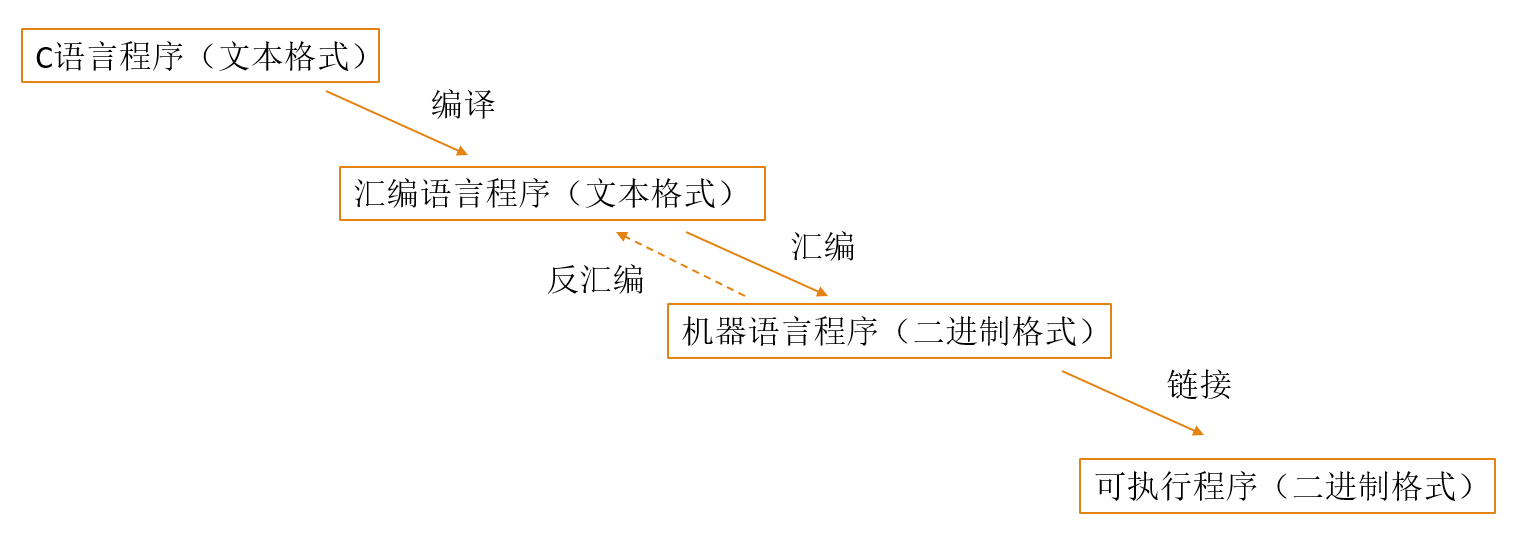
\includegraphics[width = 1\textwidth]{figure/LecPic3-1.PNG}
            \caption{程序从C语言到机器语言的转换}
            \label{fig:my_label}
        \end{figure}
        
        \item    汇编语言程序
            \begin{itemize}
            \item 汇编代码不区分有无符号整数、各种类型的指针,甚至不区分指针和整数
            \item 返回指令后插入一些无影响的指令是为了将函数机器代码变为16字节,方便存储
            \item 以“.”开头的伪指令可以忽略
            \end{itemize}
        
        \item  机器语言程序
            \begin{itemize}
            \item 机器执行的程序只是一个字节序列。
            \end{itemize}
            
        \item 汇编与反汇编
            \begin{itemize}
            \item 反汇编器的指令命名规则和编译器生成的汇编代码有细微差别
            \item 常用指令及操作数较少的指令所需字节数少,反之则所需字节数多
            \end{itemize}
        
        
        
    \end{enumerate}  
    
    \subsection{机器代码中可见的处理器状态}
    \begin{itemize}
        \item 程序计数器(PC,\%rip):给出将要执行的下一条指令在内存中的地址
        \item 整数寄存器:16个64位存放指针或整数数据(如过程参数、局部变量和函数返回值)
        \item 条件码寄存器:保存最近执行的算术或逻辑指令的状态信息,实现if/while等结构
        \item 向量寄存器:存放整数数据和浮点数据

    \end{itemize}
        
    \section{认识寄存器}
    \begin{enumerate}
        \item 
    \end{enumerate}
    
    
    
    
    
    
\end{document}